\documentclass[11pt]{article}
\usepackage{latexsym}
\usepackage{amsmath}
\usepackage{amssymb}
\usepackage{amsthm}
\usepackage{epsfig}
\usepackage[tight]{subfigure}
\usepackage{subcaption}
\usepackage{amsmath}

\DeclareMathOperator*{\minimize}{min}
\DeclareMathOperator*{\maximize}{max}

\usepackage{algorithm}
 %on linux you may need to run sudo apt-get install texlive-full to install algorithm.sys
\usepackage{algorithmic}
\renewcommand{\algorithmiccomment}[1]{\hfill //~#1\normalsize}
\usepackage{verbatim}

\newcommand{\handout}[5]{
  \noindent
  \begin{center}
  \framebox{
    \vbox{
      \hbox to 5.78in { {#1} \hfill #2 }
      \vspace{4mm}
      \hbox to 5.78in { {\Large \hfill #5  \hfill} }
      \vspace{2mm}
      \hbox to 5.78in { {\em #3 \hfill #4} }
    }
  }
  \end{center}
  \vspace*{4mm}
}

\newcommand{\lecture}[5]{\handout{#1}{#2}{#3}{#4}{#5}}
\newcommand{\collision}[0]{\mathrm{collision}}
\newcommand{\nocollision}[0]{\overline{\collision}}

\newcommand*{\QED}{\hfill\ensuremath{\square}}

\newtheorem{theorem}{Theorem}
\newtheorem{corollary}[theorem]{Corollary}
\newtheorem{lemma}[theorem]{Lemma}
\newtheorem{observation}[theorem]{Observation}
\newtheorem{proposition}[theorem]{Proposition}
\newtheorem{definition}[theorem]{Definition}
\newtheorem{claim}[theorem]{Claim}
\newtheorem{fact}[theorem]{Fact}
\newtheorem{assumption}[theorem]{Assumption}
\newtheorem{note}[theorem]{Note}

% 1-inch margins, from fullpage.sty by H.Partl, Version 2, Dec. 15, 1988.
\topmargin 0pt
\advance \topmargin by -\headheight
\advance \topmargin by -\headsep
\textheight 8.9in
\oddsidemargin 0pt
\evensidemargin \oddsidemargin
\marginparwidth 0.5in
\textwidth 6.5in

\parindent 0in
\parskip 1.5ex
%\renewcommand{\baselinestretch}{1.25}

\begin{document}

\lecture{Statistical Techniques in Robotics (16-831, S20)}{Lecture \#16
  (Wednesday, May 31)}{Lecturer: Kris Kitani}{Scribes: Jeet Kanjani, Shubham Gupta}{Model Based Reinforcement Learning}

\section{Review}
    \begin{flushleft}
    \subsection*{Markov Decision Process}
    A Markov Decision Process is a mathematical framework for describing a fully observable environment where the outcomes are partly random and partly under control of the agent. \cite{concina} At every timestep, the agent samples an action from policy (distribution) $\pi(a|x)$, and uses the state transition probability $p(s'|s,a)$ to determine the next state s'. The stochastic nature of the environment causes the agent to be in different states given the current state and action. The reward agent recieves at every timestep is denoted by $r(s',s,a)$. A markov decision process can be represented as a graphical model:
    
    \begin{figure}[H]
        \centering
        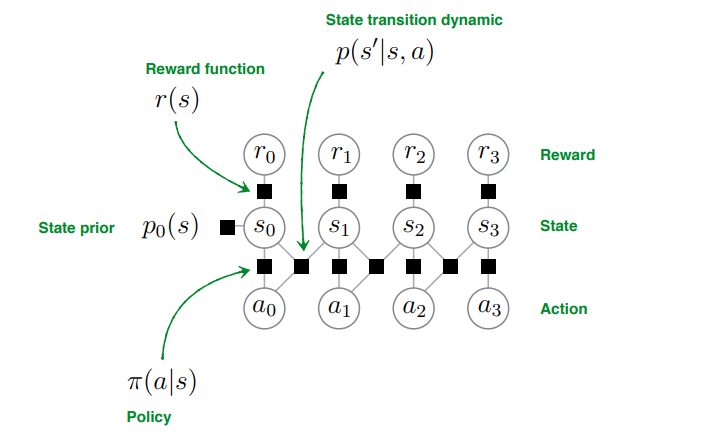
\includegraphics[scale = 0.45]{images/MDP.png}
        \caption{Markov Decision Process}
        \label{fig:my_label}
    \end{figure}
        This factorization of this model can be written as:
        \begin{equation}
        p\left(s_{0}, s_{1}, a_{1}, \cdots, s_{T}\right)=p_{0}\left(s_{0}\right) \prod_{t} p\left(s_{t+1} \mid s_{t}, a_{t}\right) p\left(a_{t} \mid s_{t}\right)        
    \end{equation}
    In RL, we try to maximize the cumulative reward over a sequence of states and actions. In model based RL, we have access to the $p(s'|s,a)$ and the reward function which we can use to learn a policy $\pi(a|x)$ that maximizes the cumulative reward.
    \\   
    
\end{flushleft}
    \subsection*{Value Function}
    The value function represents how good is a state for an agent to be in. It is equal to the expected total reward for the agent starting from state s. The value function depends on the policy by which the agent picks actions to perform.\cite{Moustafa} The state-action value is given by:
    $$
Q^{\pi}(s, a)=\mathbb{E}_{p}\left[\gamma^{0} r\left(s_{0}\right)+\gamma^{1} r\left(s_{1}\right)+\gamma^{2} r\left(s_{2}\right)+\cdots \mid s_{0}=s, a_{0}=a\right]
$$
The relationship between the state value function and state-action value function is given by:
$$
V^{\pi}(s)=\sum_{a} \pi(a \mid s) Q^{\pi}(s, a)
$$






%This section serves as a review of the previous lecture and any other context required to frame the content of the current lecture. 

%You may format the scribes in any way you like, aside from changing font style, size, and page format. Please use subsections and paragraphs to increase the readability of your notes.

%Length requirement 1-2 pages.
        

\section{Summary}
\subsection{Bellman Optimality Equation}
The state-value function is a linear combination of the immediate reward $r_{t}$ plus the discounted reward of the next state. This results in a recursive relationship between state value functions for a given policy:
$$
V^{\pi}(s)=\mathbb{E}_{p}\left[r_{t}+\gamma V^{\pi}\left(s_{t+1}\right) \mid s_{t}=s\right]
$$
This can be interpreted as future rewards i.e. value obtained after taking an action and receiving a reward. The relationship between state-action value functions that can be obtained is known as the Bellman equation.
$$
Q^{\pi}(s, a)=\mathbb{E}_{p}\left[r_{t}+\gamma Q^{\pi}\left(s_{t+1}, a_{t+1}\right) \mid s_{t}=s, a_{t}=a\right]
$$


This gives us the methods to derive the Bellman optimality equations. When comparing two policies, the policy with the better value function should give a better return.
$$
\begin{aligned}
V^{\pi^{*}}(s) &=\max _{\pi} V^{\pi}(s) \\
Q^{\pi^{*}}(s, a) &=\max _{\pi} Q^{\pi}(s, a)
\end{aligned}
$$


We get a recursive relation when we substitute the expectation into the previous expectation. This is the Bellman Optimality equation:
$$
\begin{array}{c}
V^{\pi^{*}}(s)=\max _{a} \sum_{s^{\prime}} p\left(s^{\prime} \mid s, a\right)\left[r_{t}+\gamma V^{\pi^{*}}\left(s^{\prime}\right)\right] \\
Q^{\pi^{*}}(s, a)=\sum_{s^{\prime}} p\left(s^{\prime} \mid s, a\right)\left[r(s)+\gamma \max _{a^{\prime}} Q^{\pi^{*}}\left(s^{\prime}, a^{\prime}\right)\right]
\end{array}
$$

The proof of the above equation is given in the appendix.

\subsection*{Computing the optimal policy}
The goal of reinforcement learning is to learn the policy which maximizes the expected return. 

\begin{equation}
    \hat{\pi}=\underset{\pi}{\arg \max } \mathbb{E}_{p_{\pi}(\zeta)}\left[\sum_{t=0}^{T} r^{(t)}\right]
\end{equation}

Since the policy can be derived from the state-action value function, we just need the value function to obtain the optimal policy. 
This is called value-based reinforcement learning where we iteratively try to find the optimal value function which would entail an optimal policy.

\begin{figure}[H]
    \centering
    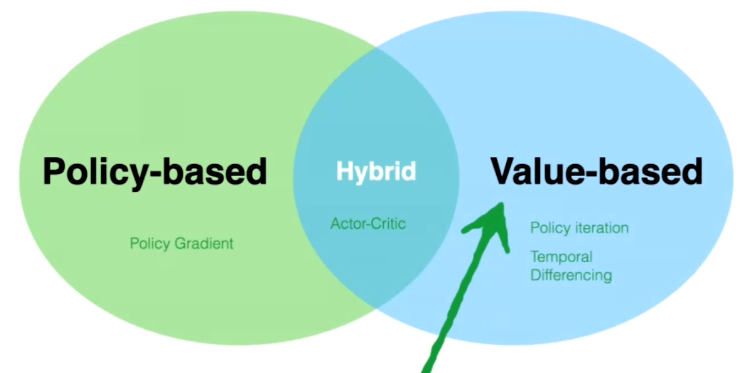
\includegraphics[scale=0.4]{images/types of RL.png}
    \label{fig:my_label}
\end{figure}

\begin{equation}
    \pi(s)=\underset{a}{\arg \max } Q(s, a)
\end{equation}

In RL, the task of \textbf{Prediction} is referred to as the task to solve for the optimal policy.

\\ 
There are two types of prediction methods depending on what is assumed for the environment.

\begin{itemize}
    \item \textbf{Model Based}: Model is fully specified (Access to inner working of the environment)
    \item \textbf{Model-free} Model is limited to interactions
\end{itemize}
\subsection{RL Approaches for Optimal Policy}
The various approaches to solve RL can be divided in 3 categories:
\begin{itemize}
    \item \textbf{Policy-based:} These methods build an explicit policy representation. Eg - policy gradients  
    \item \textbf{Value-based:} These methods use value functions to derive the optimal policy (implicit representation). Eg- policy iteration, temporal differencing 
    \item \textbf{Hybrid:} Mix of above 2. Eg- actor critic
\end{itemize}
We will solve the value-based model based RL in the next section.
\newpage
\subsection{Value-based Model-based RL}
\subsubsection{Chicken and Egg Problem}
In order to find the optimal policy using the value function, we can use the Bellman optimality equation. \\ Let's formalize this mathematically. We have 
\begin{itemize}
    \item Finite state space $s \in S$
    \item Finite action space $a \in A$
    \item State transition dynamics $p(s^{'}|s,a)$
    \item Reward function $r(s^{'},a,s)$
\end{itemize}

We need to estimate the value function $V^{\pi} (s)$ or $Q^{\pi}(s, a)$ which in turn can be used to find the optimal policy $\pi^{*}$ using the Bellman optimality equation. Problem is that in order to estimate the value function we also need the policy $\pi(a|s)$. Now, this becomes like a chicken and egg problem where we want to find the optimal policy using the value function but the value function estimation also needs policy.
\subsubsection{Policy Iteration}
The above-stated chicken and egg problem can be solved iteratively. We can start with an initial guess for policy, compute the value function for this policy using the Bellman equation, and use the Bellman optimality equation to find a new optimal policy for this value function. We can keep on doing this iteratively till convergence is met. \\
\begin{figure}[H]
    \centering
    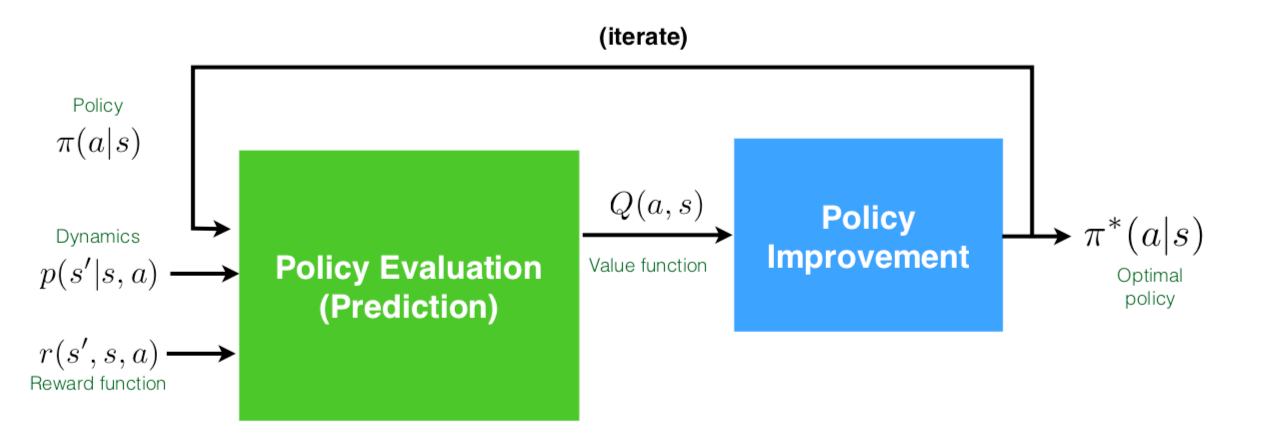
\includegraphics[scale=0.4]{images/value_based.png}
    \caption{Policy Iteration Method for RL}
\end{figure}
Here the step to estimate the value function is called the Policy Evaluation (Prediction). The estimation of the optimal policy is called Policy Improvement. \\

\subsubsection{Policy Evaluation a.k.a Prediction}
The prediction block is the most important block in model-based RL methods. This block takes as input the current policy, state transition dynamics, and reward function and derives the optimal value function by recursion. Since it involves multiple iterations over all the possible action and state space, it is a highly computationally expensive block. 
\begin{figure}[H]
    \centering
    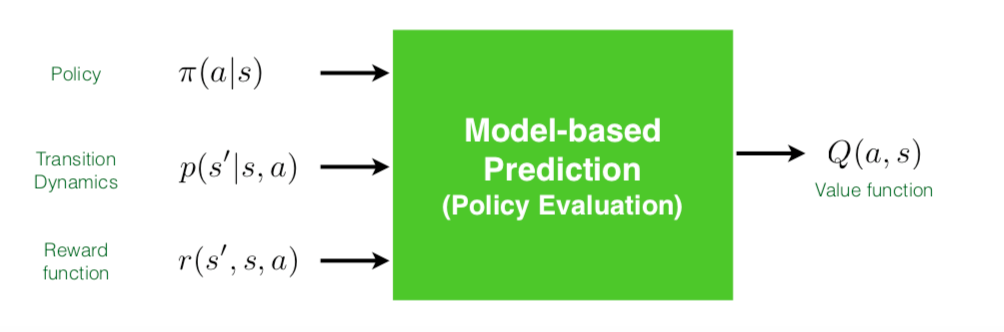
\includegraphics[scale=0.4]{images/prediction.png}
    \caption{Policy Evaluation Block}
\end{figure}

\subsubsection{Policy Improvement}
Given a value function, the policy improvement block finds the optimal policy using the Bellman optimality equation. This can be simply computed by finding the optimal action for each of the possible states using the value function. \\
\begin{figure}[H]
    \centering
    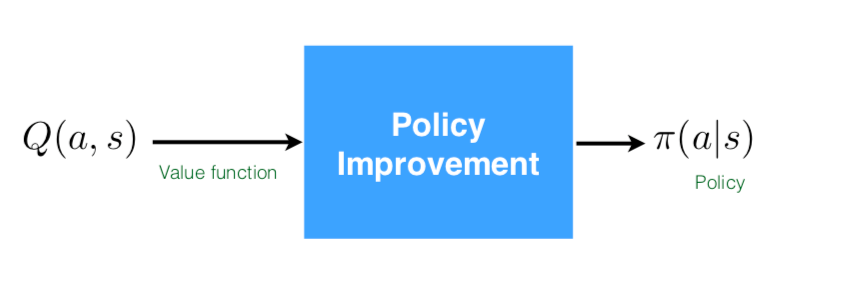
\includegraphics[scale=0.4]{images/improvement.png}
    \caption{Policy Improvement Block}
\end{figure}
\newpage
\subsubsection{Algorithm}
We can formalize the above approach in the form of a pseudo-code mentioned below. \\

	\begin{algorithm}[H]
	\caption{function POLICYITERATION $\left(r(s), p\left(s^{\prime} \mid s, a\right), \gamma\right)$}
    \begin{algorithmic}[1]
    \STATE $\pi \leftarrow \operatorname{rand}(\mathcal{A})$
    \STATE $V \leftarrow \operatorname{rand}(\mathbb{R})$
    \STATE $V^{\prime} \leftarrow \operatorname{rand}(\mathbb{R})$
    \WHILE{$\max _{s}\left|V(s)-V^{\prime}(s)\right| \geq \epsilon$}
    \STATE $V^{\prime} \leftarrow V$
    \FOR{$s \in \mathcal{S}$}
    \STATE $Q(s, a)=r(s)+\gamma \sum_{s^{\prime}} p\left(s^{\prime} \mid s, a\right) V^{\prime}\left(s^{\prime}\right) \quad \forall a$
    \STATE $V(s)=\sum_{a} \pi(a \mid s) Q(s, a)$
    \ENDFOR
    \ENDWHILE
    \FOR{$s \in \mathcal{S}$}
    \STATE $\pi^{\prime}(s)=\arg \max _{a} Q(s, a)$
    \ENDFOR
    \IF{$\pi^{\prime}=\pi$}
    \STATE return $\pi$
    \ENDIF
    \STATE Go to line 2
    \end{algorithmic}
	\end{algorithm}

\subsection{Computational Optimization}
We can represent the above algorithm graphically as shown below. \\
\begin{figure}[H]
    \centering
    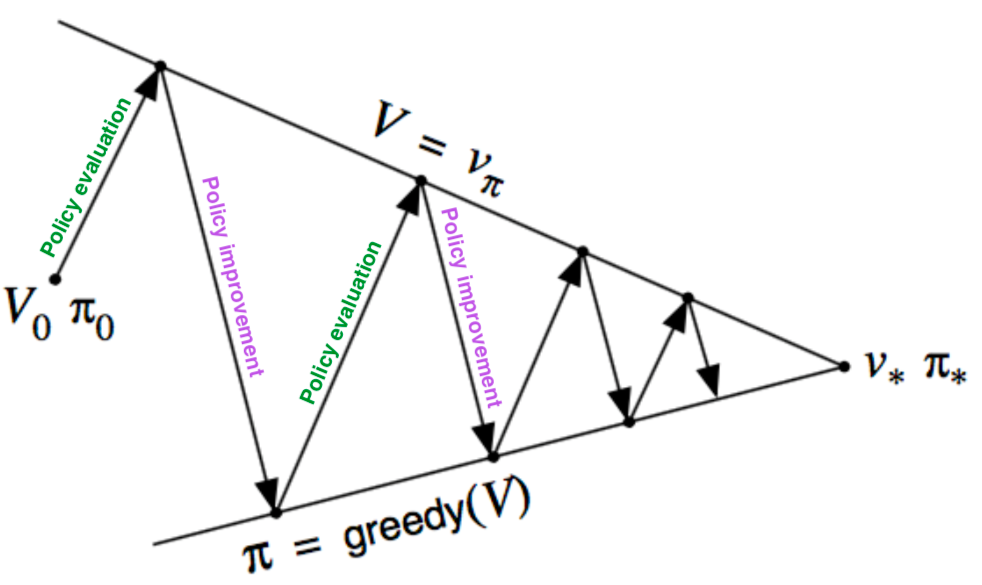
\includegraphics[scale=0.35]{images/policy_iteration.png}
    
\end{figure}
Here, we can observe that we need to perform multiple iterations to compute the value function at each given policy before updating the current policy. Instead of doing this, we can actually keep on updating the policy each time we estimate a new value function. This can be thought of as applying stochastic gradient descent in place of batch gradient descent for faster convergence.
\subsubsection{Value iteration}
The above-mentioned idea of simultaneously updating the policy and value function is called value iteration. 
	\begin{algorithm}[H]
	\caption{function VALUEITERATION $\left(r(s), p\left(s^{\prime} \mid s, a\right), \gamma\right)$}
    \begin{algorithmic}[1]
    \STATE $\pi \leftarrow \operatorname{rand}(\mathcal{A})$
    \STATE $V \leftarrow \operatorname{rand}(\mathbb{R})$
    \STATE $V^{\prime} \leftarrow \operatorname{rand}(\mathbb{R})$
    \WHILE{$\max _{s}\left|V(s)-V^{\prime}(s)\right| \geq \epsilon$}
    \STATE $V^{\prime} \leftarrow V$
    \FOR{$s \in \mathcal{S}$}
    \STATE $Q(s, a)=r(s)+\gamma \sum_{s^{\prime}} p\left(s^{\prime} \mid s, a\right) V^{\prime}\left(s^{\prime}\right) \quad \forall a$
    \STATE $\pi^{\prime}(s)=\arg \max _{a} Q(s, a)$
    \STATE $V(s)=\sum_{a} \pi(a \mid s) Q(s, a)$
    \ENDFOR
    \ENDWHILE
    \IF{$\pi^{\prime}=\pi$}
    \STATE return $\pi$
    \ENDIF
    \STATE Go to line 2
    \end{algorithmic}
	\end{algorithm}

As shown in the below figure, the value iteration method converges much faster in comparison to the sequential update method.
\begin{figure}[H]
    \centering
    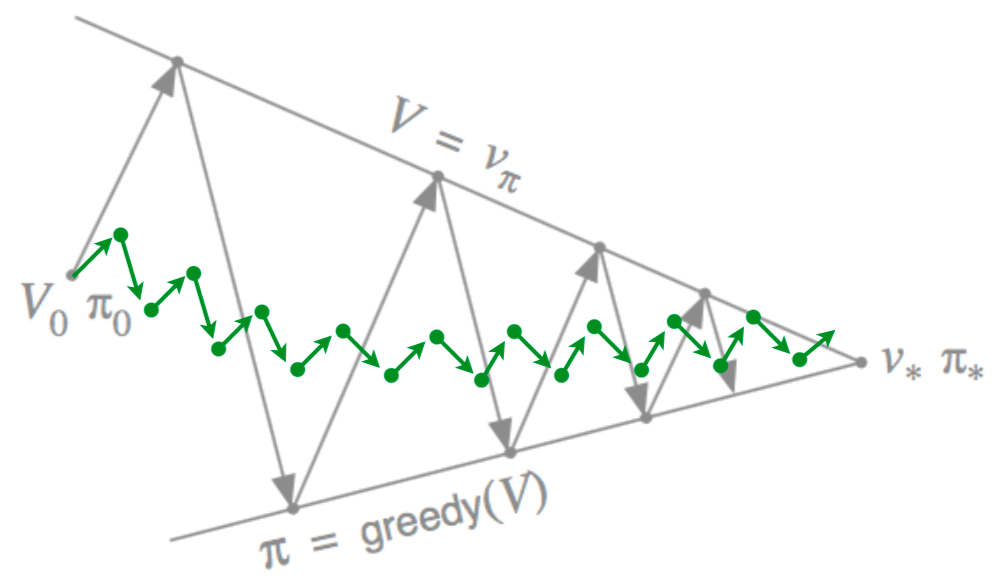
\includegraphics[scale=0.4]{images/value_iteration.png}
    
\end{figure}

%\section*{References}
%Include your references here. Please cite any resources you found useful.	
%Populate the refs.bib file or list your references manually. Be consistent in formatting!



{
\bibliography{refs}
\bibliographystyle{abbrv}
\begin{thebibliography}{9}
    
    \bibitem{concina} 
    F Concina Reinforcement Learning - Markov Decision Process\\
    [\textit{[Markov Decision Process](https://fabioconcina.github.io/blog/markov-decision-process)}]
    \bibitem{Moustafa} 
    
    Deep Reinforcement Learning Demystified - Policy Iteration, Value Iteration and Q learning\\
    [\textit{https://medium.com/@m.alzantot/deep-reinforcement-learning-demysitifed-episode-2-policy-iteration-value-iteration-and-q-978f9e89ddaa}]
\end{thebibliography}

}


%\section{Appendix}
%This section provides any relevant background material that was not covered in the lectures but was found to be useful for understanding the material. 
%For example, derivations, theory underlying techniques employed, etc. 

%Additionally, this section can summarize applications or extensions of these techniques found in the literature. 
\subsection{Appendix}
Proof for Bellman Optimality equation:
\begin{equation}
\begin{aligned}
V^{\pi^{*}}(s) &=\sum_{a} \pi(a \mid s) Q^{\pi^{*}}(s, a) \\
&=\max _{a} Q^{\pi^{*}}(s, a) \\
&=\max _{a} \mathbb{E}\left[\sum_{t=0}^{\infty} \gamma^{t} r_{t} \mid s_{0}=s, a_{0}=a\right] \\
&=\max _{a} \mathbb{E}\left[r_{0}+\sum_{t=1}^{\infty} \gamma^{t} r_{t} \mid s_{0}=s, a_{0}=a\right] \\
&=\max _{a} \sum_{s^{\prime}} p\left(s_{1}=s^{\prime} \mid s, a\right)\left[r_{0}+\mathbb{E}\left\{\sum_{t=1}^{\infty} \gamma^{t} r_{t} \mid s_{1}=s^{\prime}\right\}\right]
\end{aligned}
\end{equation}
\end{document} % Done!


